\begin{multicols}{2}
    \section*{Введение}
    \normalsize{Современные компьютеры, несмотря на все их чудеса, работают по тому же фундаментальному принципу, что и механические устройства, придуманные Чарльзом Бэббиджем в 19 веке и позже формализованные Аланом Тьюрингом: одно стабильное состояние машины представляет одно число. Даже, казалось бы, нестандартные вычислительные модели, такие как модель, основанная на ДНК, разделяют этот основной принцип. Тем не менее физики показали, что законы, описывающие мир природы, ~--- это не простые законы классической механики, а более тонкие законы квантовой физики, и они побуждают нас по-другому думать о вычислениях \ldots
    
    Цифровые электронные компьютеры, широко используемые в настоящее время, созданы с помощью полупроводниковых технологий. Такие компьютеры обычно представляют собой совокупность элементов только с двумя возможными логическими состояниями <<0>> и <<1>>~--- так называемых битов (binary digits = bits), вентильных элементов, и соединений между ними. Такие компьютеры, в которых логические операции производятся с этими классическими, с точки зрения физики, состояниями, в настоящее время принято называть \emph{классическими}.

    Однако уже достаточно давно было обнаружено, что эти классические компьютеры не могут справиться с некоторыми очень важными задачами. Примерами таких задач являются поиск в неструктурированной базе данных, моделирование эволюции квантовых систем (например, ядерные реакции) и, наконец, факторизация больших чисел.

    Интерес к последней задаче связан с тем, что практически все современные шифры для секретной переписки основаны на этой математической процедуре.

    Для взлома уже существующего кода необходима работа классического компьютера в течении нескольких лет. Предполагаемое экспоненциальное увеличение счёта в случае возникновения квантового компьютера сильно встревожило <<секретное>> мировое сообщество, и оно стала вкладывать немалые средства в исследования и разработки в области квантового компьютера и квантовых вычислений.}
    \section*{Квантовые биты}
    \normalsize{Бит~--- это фундаментальное понятие классических вычислений и классической информации.
    Квантовые вычисления и квантовая информация построены на аналогичной концепции~---
    квантовом бите, или сокращенно кубите. В этом разделе мы познакомимся со свойствами одиночных
    кубитов, сравнивая и противопоставляя их свойства свойствам классических битов.
    
    Что такое кубит? Мы собираемся описать кубиты как математические объекты с определенными
    специфическими свойствами. <<Но подождите,~--- скажете вы,~--- я думал, кубиты~--- это физические объекты>>. Это верно, что кубиты, как и биты, реализуются как реальные физические системы, между абстрактной математической точкой зрения и реальными системами существует связь.
    Однако по большей части мы рассматриваем кубиты как абстрактные математические объекты. Прелесть рассмотрения кубитов как абстрактных сущностей заключается в том, что это
    дает нам свободу в построении общей теории квантовых вычислений и квантовой
    информации, реализация которой не зависит от конкретной системы.
    Что же тогда такое кубит? Точно так же, как классический бит имеет состояние~--- либо 0, либо 1,~--- кубит также имеет состояние. Двумя возможными состояниями для кубита являются состояния $\vert$0$\rangle$ и $\vert$1$\rangle$, которые, как вы могли
    догадаться, соответствуют \emph{состояниям} 0 и 1 для классического бита. Обозначение типа <<$\vert$~$\rangle$>> называется \emph{обозначением Дирака}, и мы будем часто его видеть, поскольку это стандартное обозначение состояний в квантовой механике. Разница между битами и кубитами заключается в том, что кубит может находиться в \emph{состоянии}, отличном от $\vert$0$\rangle$ или $\vert$1$\rangle$ . Также возможно формировать \emph{линейные комбинации} состояний, часто называемые \emph{суперпозициями}:
    \begin{equation}
        \vert\psi\rangle = \alpha\vert0\rangle + \beta\vert1\rangle,
    \end{equation}
    где $\alpha$ и $\beta$ ~--- комплексные числа.
    Способность кубита находиться в состоянии суперпозиции противоречит нашему
    пониманию окружающего нас физического мира, основанному на <<здравом смысле>>. Классический бит подобен монете: либо орлом, либо решкой вверх. Для несовершенных монет могут существовать промежуточные состояния, такие как балансирование на ребре, но в идеальном случае ими можно пренебречь. Напротив, кубит может существовать в континууме состояний между $\vert$0$\rangle$ и $\vert$1$\rangle$~--– до тех пор, пока его не будут наблюдать. Давайте еще
    раз подчеркнем, что когда измеряется кубит, он всегда выдает только <<0>> или <<1>> в качестве результата измерения. Например, кубит может находиться в состоянии
    \begin{equation}
        \frac{1}{\sqrt{2}}\vert0\rangle+\frac{1}{\sqrt{2}}\vert1\rangle,
    \end{equation}
    что при измерении дает результат 0 в половине случаев ($\vert1/\sqrt{2}\vert^2$) и результат 1 в половине случаев.
    Несмотря на эту странность, кубиты определенно реальны, их существование и поведение полностью подтверждены экспериментами (Опыт Штерна--Герлаха), и для реализации кубитов можно использовать множество различных физических систем.
    
    Чтобы получить конкретное представление о том, как
    может быть реализован кубит, полезно перечислить некоторые из способов, которыми эта реализация может произойти: две разные поляризации фотона; выравнивание ядерного спина в
    однородном магнитном поле; два состояния электрона, вращающегося вокруг одного атома, как показано на рис. 1. В модели атома электрон может существовать либо в так называемом <<основном>>, либо в <<возбужденном>> состояниях, которые мы будем называть $\vert0\rangle$ и $\vert1\rangle$ соответственно. Направляя свет на атом
    с соответствующей энергией и в течение соответствующего промежутка времени, можно перевести
    электрон из состояния $\vert0\rangle$ в состояние $\vert1\rangle$ и наоборот. Но что еще более интересно, сокращая время, в течение которого мы излучаем свет, электрон, изначально находящийся в состоянии $\vert0\rangle$, может быть перемещен
    <<на полпути>> между $\vert0\rangle$ и $\vert1\rangle$, в состояние $\vert+\rangle$.
    }
    \begin{center}
    \begin{minipage}{0.3\textwidth}{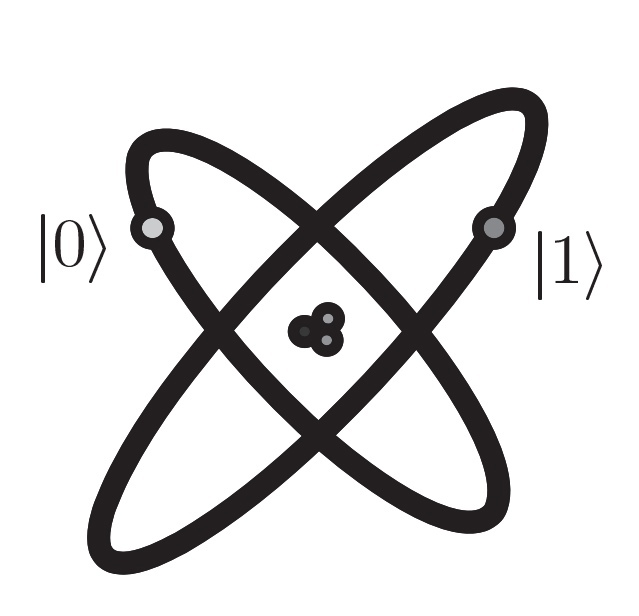
\includegraphics[scale=0.2]{qubit_1.jpg}}
    \end{minipage}\\
    \vspace{0.3cm}
    \footnotesize{\textbf{Рисунок 1.} Кубит, представленный двумя электронными уровнями в атоме.}
    \end{center}
    \normalsize{
    Так как \(\vert\alpha^2\vert + \vert\beta^2\vert = 1\), мы можем записать равенство (1) следующим образом:
    }
    \begin{equation}
        \vert\psi\rangle=e^{i\gamma}\Bigg(\cos\frac{\theta}{2}\vert0\rangle+e^{i\phi}\sin\frac{\theta}{2}\vert1\rangle\Bigg),
    \end{equation}
    \normalsize{
    где $\theta,~\phi$ и $\gamma$~--- действительные числа. На самом деле мы можем не учитывать влияние $e^{i\gamma}$ из-за отсутствия \emph{заметных эффектов}, что позволит нам записать это выражение в следующем виде:
    }
    \begin{equation}
        \vert\psi\rangle=\cos\frac{\theta}{2}\vert0\rangle+e^{i\phi}\sin\frac{\theta}{2}\vert1\rangle.
    \end{equation}
    \normalsize{
    Числа $\theta$ и $\phi$ определяют точку на единичной трехмерной сфере, как показано на рис. 2. Эту сферу часто называют сферой Блоха (названной в честь Феликса Блоха).
    Она обеспечивает хорошую визуализацию состояния отдельного кубита и часто служит отличным испытательным стендом для идей о квантовых вычислениях и квантовой информации. Многие операции над одним
    кубитом четко описаны в рамках сферы Блоха. Однако следует иметь в виду, что не существует обобщения сферы Блоха на множество кубитов.
    }
    \begin{center}
    \begin{minipage}{0.3\textwidth}{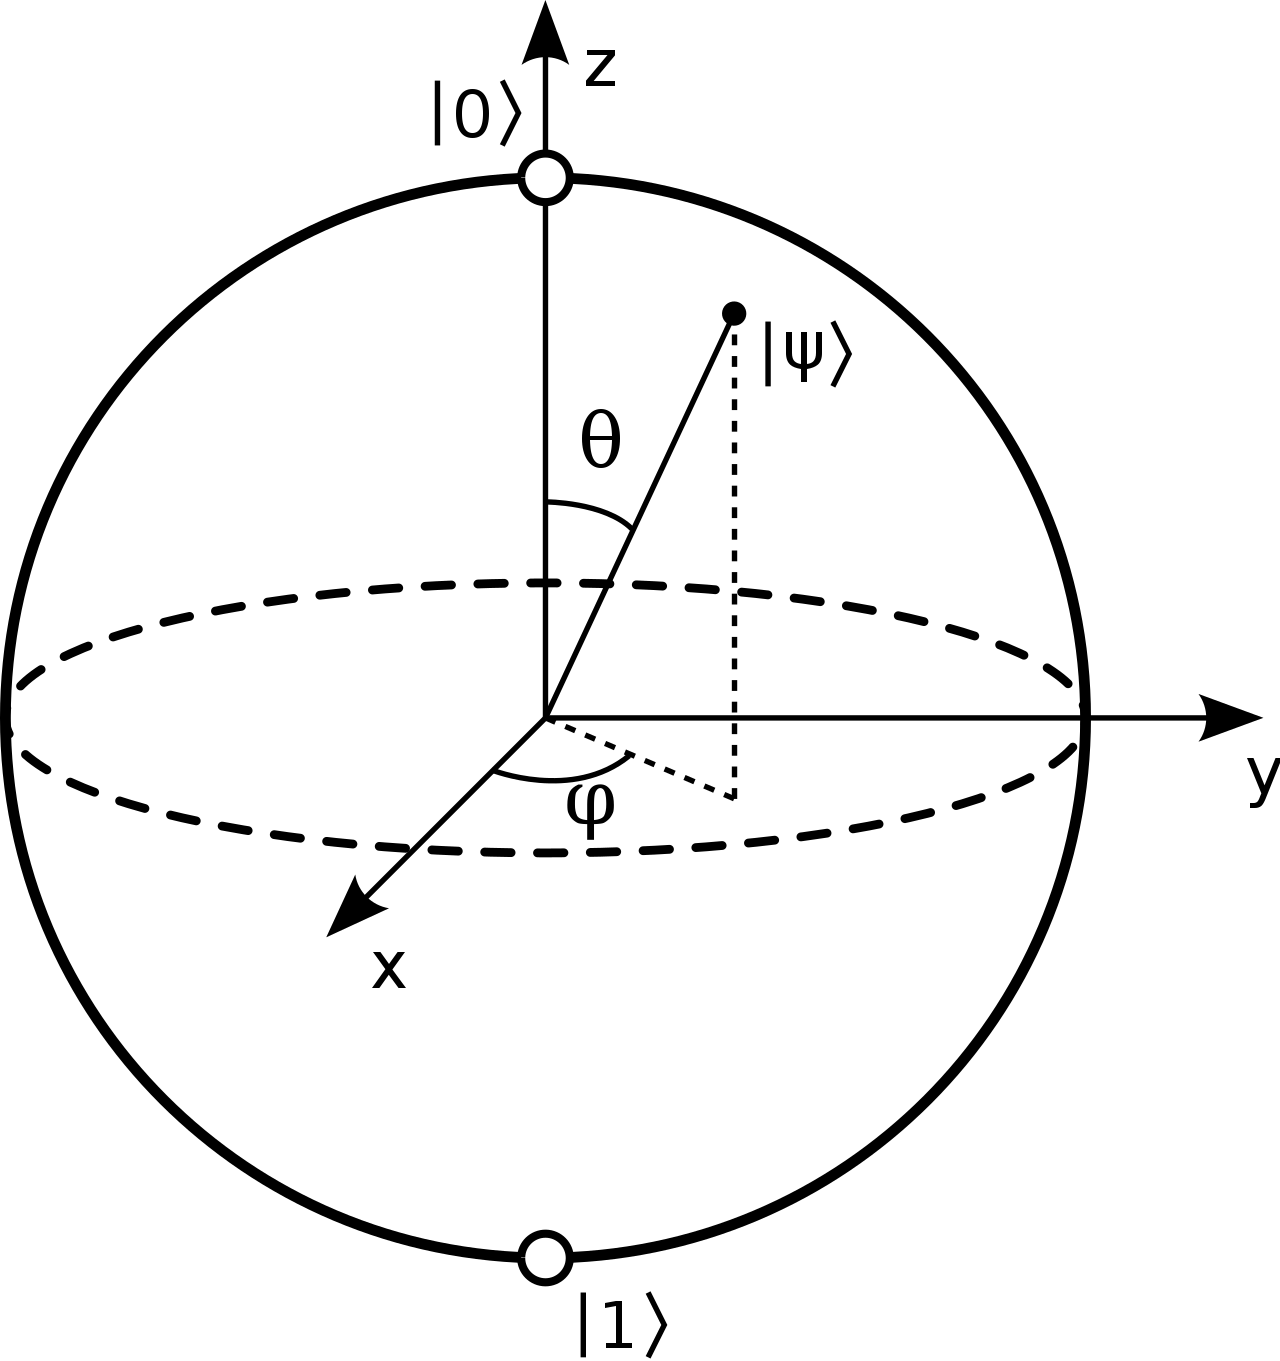
\includegraphics[scale=0.15]{Bloch_sphere.png}}
    \end{minipage}\\
    \vspace{0.3cm}
    \footnotesize{\textbf{Рисунок 2.} Преставление кубита в виде сферы Блоха.}
    \end{center}
    \normalsize{
    Какой объем информации представлен кубитом? Парадоксально,
    но на единичной сфере существует бесконечное число точек, так что в принципе можно было бы сохранить весь текст Шекспира в бесконечном двоичном разложении $\theta$. Однако этот вывод
    является заблуждением из-за поведения кубита при наблюдении. Напомним, что
    измерение кубита даст \emph{только} либо 0, либо 1. Кроме того, измерение \emph{изменяет}
    состояние кубита, переводя его из суперпозиций $\vert0\rangle$ и $\vert1\rangle$ в конкретное состояние,
    соответствующее результату измерения. Например, если измерение $\vert+\rangle$ дает 0,
    то состояние кубита после измерения будет равно $\vert0\rangle$. Почему такое происходит? Никто не знает. Такое поведение является одним из \emph{фундаментальных постулатов} квантовой механики. Что важно для наших целей, так это то, что в результате одного измерения можно получить только один бит информации о состоянии кубита, разрешая таким образом кажущийся парадокс. Оказывается, что только в том случае, если было измерено бесконечно много одинаковых подготовленных кубитов, можно было бы определить $\alpha$ и $\beta$ для кубита в состоянии, заданном в уравнении (1).
    Но еще более интересным является вопрос: какой объем информации
    представлен кубитом, если \emph{мы его не измеряем}? Это вопрос с подвохом, потому что как
    можно количественно оценить информацию, если ее нельзя измерить? Тем не менее, здесь есть нечто
    концептуально важное, потому что, когда Природа развивает замкнутую квантовую систему
    кубитов, не выполняя никаких <<измерений>>, она, по-видимому, отслеживает все
    непрерывные переменные, описывающие состояние, такие как $\alpha$ и $\beta$. В некотором смысле, в состоянии кубита Природа скрывает огромное количество <<скрытой информации>>. И что еще более интересно, потенциальный объем этой дополнительной <<информации>> растет экспоненциально с
    увеличением количества кубитов. Понимание этой скрытой квантовой информации~--- это вопрос, который лежит в основе того, что делает квантовая механика~--- мощный инструмент для обработки информации.
    }
    \section*{Множества кубитов}
    \normalsize{
    Рассмотрим систему из $n$ кубитов. Вычислительные базовые состояния этой системы имеют вид \(\vert x_1x_2\ldots x_n\rangle\), и поэтому квантовое состояние такой системы задается $2^n$ амплитудами.
    Для $n = 500$ это число больше, чем предполагаемое количество атомов во Вселенной! Попытка сохранить все эти комплексные числа была бы невозможна
    ни на одном классическом компьютере. Гильбертово пространство действительно большое.
    Однако Природа манипулирует такими огромными объемами данных даже для
    систем, содержащих всего несколько сотен атомов. Это похоже на то, как если бы Природа хранила $2^{500}$
    бумажек, на которых она выполняет свои вычисления по мере развития системы.
    Эта огромная потенциальная вычислительная мощность~--- то, чем мы бы очень
    хотели воспользоваться. Но как мы можем думать о квантовой механике как о вычислении?
    
    \emph{Изменения}, происходящие в квантовом состоянии, могут быть описаны с помощью языка квантовых
    вычислений. Аналогично тому, как классический компьютер строится из электрической схемы, содержащей провода и логические элементы, квантовый компьютер строится из \emph{квантовой схемы}, содержащей провода и элементарные квантовые элементы для переноса
    квантовой информации и манипулирования ею.
    }\\
    \section*{Однокубитные вентили}
    \normalsize{
        Классические компьютерные схемы состоят из проводов и логических элементов. Провода используются для передачи
        информации по схеме, в то время как логические элементы выполняют манипуляции с информацией, преобразуя ее из одной формы в другую. Рассмотрим, например, классические однобитовые
        логические элементы. Единственным нетривиальным членом этого класса является элемент NOT, работа
        которого определяется его таблицей истинности, в которой 0 → 1 и 1 → 0, то есть состояния 0 и 1
        меняются местами.

        Можно ли определить аналогичный квантовый элемент NOT для кубитов? Представьте, что у нас был
        какой"=то процесс, который перевел состояние $\vert0\rangle$ в состояние $\vert1\rangle$, и наоборот.
        Такой процесс, очевидно, был бы хорошим кандидатом на квантовый аналог элемента NOT. Однако
        указание действия вентиля на состояния $\vert0\rangle$ и $\vert1\rangle$ не говорит нам, что происходит с
        суперпозициями состояний $\vert0\rangle$ и $\vert1\rangle$, без дополнительных знаний о свойствах
        квантовых вентилей. На самом деле квантовый элемент NOT действует линейно, то есть он переводит состояние
        \begin{equation}
            \alpha\vert0\rangle + \beta\vert1\rangle
        \end{equation}
        в соответствующее состояние, в котором роли $\vert0\rangle$ и $\vert1\rangle$ поменялись местами,
        \begin{equation}
            \alpha\vert1\rangle + \beta\vert0\rangle.
        \end{equation}
        Почему квантовый элемент NOT действует линейно, а не каким-то нелинейным образом "--- очень
        интересный вопрос, и ответ на него вовсе не очевиден. Оказывается, что это линейное
        поведение является общим свойством квантовой механики и очень хорошо мотивировано эмпирически;
        более того, нелинейное поведение может привести к очевидным парадоксам, таким как путешествия во времени, связь быстрее света и нарушения вторых законов термодинамики.
        Существует удобный способ представления квантового элемента NOT в матричной форме,
        который непосредственно вытекает из линейности квантовых элементов. Предположим, мы определяем матрицу
        X для представления квантового элемента NOT следующим образом:
        \begin{equation}
            X \equiv \begin{bmatrix}
            0& 1\\
            1& 0
            \end{bmatrix}.
        \end{equation}
        Если квантовое состояние $\alpha\vert0\rangle + \beta\vert1\rangle$ записано в векторной записи как
        \begin{equation}
            \begin{bmatrix}
                \alpha\\
                \beta
            \end{bmatrix},
        \end{equation}
        с верхней записью, соответствующей амплитуде для $\alpha\vert0\rangle$, а нижней 
        "--- амплитуде для $\beta\vert1\rangle$, то соответствующий выходной сигнал квантового элемента NOT равен
        \begin{equation}
            X\begin{bmatrix}
                \alpha\\
                \beta
            \end{bmatrix}
            =\begin{bmatrix}
                \beta\\
                \alpha
            \end{bmatrix}.
        \end{equation}
        Обратите внимание, что действие элемента NOT состоит в том, чтобы взять состояние $\alpha\vert0\rangle$ и заменить его состоянием
        , соответствующим первому столбцу матрицы X. Аналогично, состояние $\beta\vert1\rangle$ заменяется
        состоянием, соответствующим второму столбцу матрицы X.

        Таким образом, квантовые вентили на одном кубите могут быть описаны матрицами два на два. Существуют ли
        какие-либо ограничения на то, какие матрицы могут использоваться в качестве квантовых вентилей? Оказывается,
        так оно и есть. Напомним, что условие нормализации требует $\vert\alpha\vert^2 + \vert\beta\vert^2=1$ для квантового состояния
        $\alpha\vert0\rangle + \beta\vert1\rangle$. Это также должно быть верно для квантового состояния 
        $\vert\psi'\rangle = \alpha'\vert0\rangle+\beta'\vert1\rangle$ после срабатывания вентиля. Оказывается, что подходящим условием для матрицы, представляющей
        элемент, является то, что матрица U, описывающая элемент с одним кубитом, должна быть \emph{унитарной}, то есть $U^{\dagger} U=I$, где $U^{\dagger}$ "---
        сопряженное значение U (полученное путем транспонирования и последующего комплексного сопряжения U), а $I$ - единичная матрица два на два. Например, для элемента NOT легко
        проверить, что $X^{\dagger} X = I$.

        Удивительно, но это ограничение унитарности является единственным ограничением для квантовых вентилей. Любая
        унитарная матрица определяет допустимый квантовый элемент! Интересным следствием является то, что в
        в отличие от классического случая, когда существует только один нетривиальный элемент управления "--- элемент NOT "--- существует множество нетривиальных элементов управления с одним кубитом. Двумя важными из них 
        являются Z-вентиль:
        \begin{equation}
            Z \equiv \begin{bmatrix}
                1& 0\\
                0& -1
            \end{bmatrix},
        \end{equation}
        который оставляет $\vert0\rangle$ неизменным и меняет знак с $\vert1\rangle$ на $-\vert1\rangle$, и вентиль Адамара,
        \begin{equation}
            H\equiv \frac{1}{\sqrt2} \begin{bmatrix}
                1& 1\\
                1& -1
            \end{bmatrix}.
        \end{equation}
        Этот вентиль иногда называют <<квадратный корень из NOT>> элемента, поскольку он меняет $\vert0\rangle$ на $(\vert0\rangle + \vert1\rangle) / \sqrt2$ (первый столбец H), <<на полпути>> между $\vert0\rangle$ и $\vert1\rangle$, 
        и меняет $\vert1\rangle$ на $(\vert0\rangle - \vert1\rangle) / \sqrt2$ (второй столбец H), который также находится <<на полпути>> между $\vert0\rangle$ и $\vert1\rangle$.
        Обратите внимание, что $H^2$ не является элементом NOT, поскольку простая арифметика показывает, что $H^2 = I$, и
        , таким образом, двойное применение H к состоянию ничего с ним не делает.

        Вентиль Адамара "--- один из самых полезных квантовых вентилей, и стоит попытаться
        визуализировать его работу, рассмотрев изображение сферы Блоха. На этом рисунке (рис. 3)
        оказывается, что одиночные кубитные вентили соответствуют вращениям и отражениям сферы.
    }\\
    \begin{flushleft}
        \begin{minipage}{0.3\textwidth}{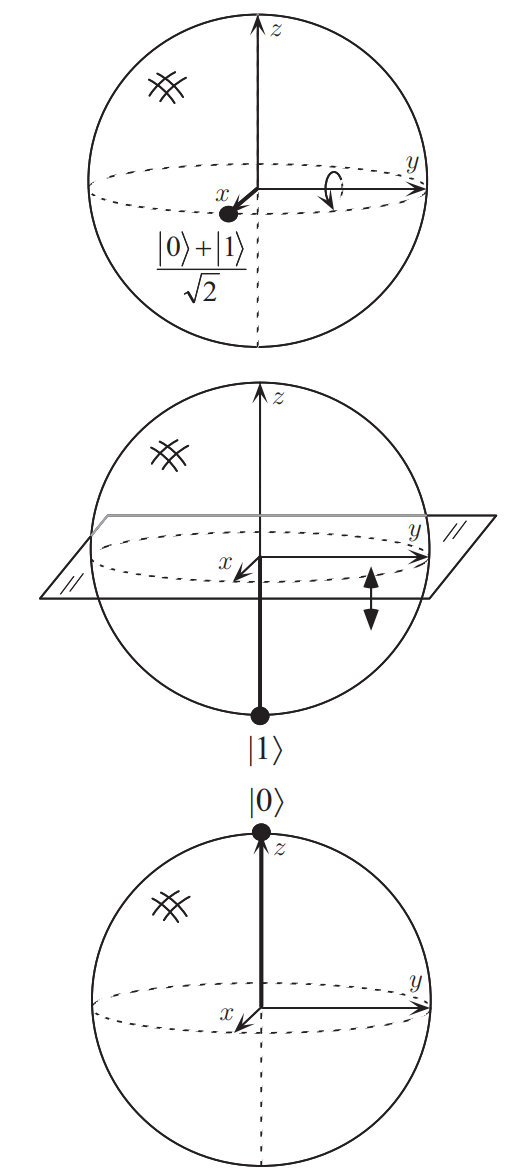
\includegraphics[scale=0.55]{Hadamard.png}}
        \end{minipage}\\
        \vspace{0.3cm}
        \footnotesize{\textbf{Рисунок 3} Визуализация вентиля Адамара на сфере Блоха, воздействующего на входное состояние $(\vert0\rangle+\vert1\rangle)/\sqrt2$.}
    \end{flushleft}
    \normalsize{
        Операция Адамара "--- это просто поворот сферы вокруг оси $\hat{y}$ на $90^{\circ}$, за которым следует
        поворот вокруг оси $\hat{x}$ на $180^{\circ}$, как показано на рис. 3.
        Некоторые важные однокубитные вентили показаны на рис. 4.
    }\\
    \begin{flushleft}
        \begin{minipage}{0.3\textwidth}{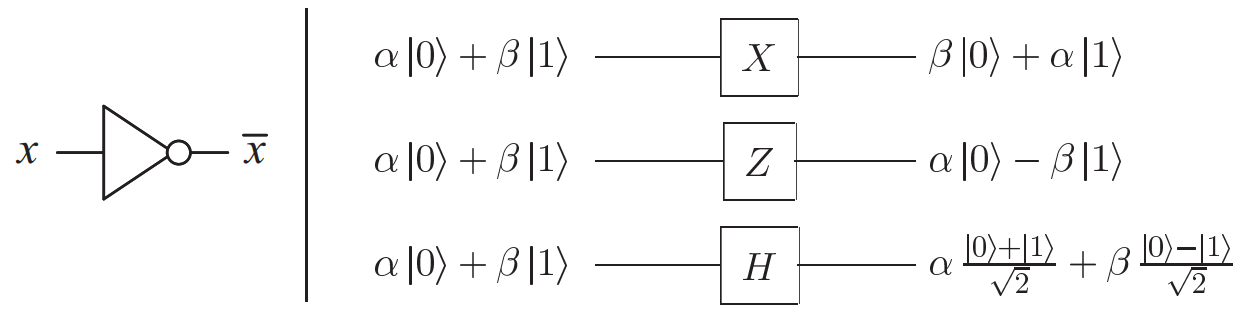
\includegraphics[scale=0.25]{Qgates.png}}
        \end{minipage}\\
        \vspace{0.3cm}
        \footnotesize{\textbf{Рисунок 4} Логические элементы с одним битом (слева) и кубитом (справа)}
    \end{flushleft}
    \normalsize{
        Существует бесконечно много унитарных матриц два на два и, следовательно, бесконечно много однокубитных вентилей. Однако оказывается, что свойства полного набора можно понять из свойств гораздо меньшего набора. Например, 
        произвольный унитарный элемент с одним кубитом может быть разложен как произведение вращений
        \begin{equation}
            \begin{bmatrix}
                \cos{\frac{\gamma}{2}}& -\sin{\frac{\gamma}{2}}\\
                \sin{\frac{\gamma}{2}}& \cos{\frac{\gamma}{2}}
            \end{bmatrix},
        \end{equation}
        и вентиль, который понимается как вращение вокруг оси $\hat{z}$,
        \begin{equation}
            \begin{bmatrix}
                e^{-i\beta/2}& 0\\
                0& e^{i\beta/2}
            \end{bmatrix},
        \end{equation}
        вместе с (глобальным) фазовым сдвигом "--- постоянным множителем формы $e^{i\alpha}$. Эти вентили
        могут быть разбиты дальше "--- нам не нужно уметь создавать эти вентили для произвольных
        $\alpha, \beta$ и $\gamma$, но можно строить сколь угодно хорошие аппроксимации для таких вентилей, используя только определенные
        специальные фиксированные значения $\alpha, \beta$ и $\gamma$. Таким образом, можно создать произвольный однокубитный вентиль, использующий конечный набор квантовых вентилей. В более общем плане, произвольное квантовое
        вычисление на любом количестве кубитов может быть сгенерировано конечным набором элементов, который, как говорят, универсален для квантовых вычислений. Чтобы получить такой универсальный набор, нам сначала нужно
        ввести некоторые квантовые вентили, включающие несколько кубитов.
    }\\
    \section*{Многокубитные вентили}
    \normalsize{
        Теперь давайте обобщим от одного до нескольких кубитов. На рисунке 5 показаны пять примечательных
        многоразрядных классических элементов управления: элементы AND, OR, XOR, NAND и NOR. Важным
        теоретическим результатом является то, что любая функция на битах может быть вычислена только из состава элементов
        NAND, которые, таким образом, известны как универсальные элементы. Напротив, XOR сам по себе или
        даже вместе с NOT не является универсальным. Один из способов увидеть это "--- отметить, что применение
        элемента XOR не изменяет общую четность битов. В результате любая схема, включающая
        только элементы NOT и XOR, если два входа x и y имеют одинаковую четность, будет выдавать выходные
        данные одинаковой четности, ограничивая класс функций, которые могут быть вычислены, и, таким образом, исключая универсальность.
    }\\
    \begin{flushleft}
        \begin{minipage}{0.3\textwidth}{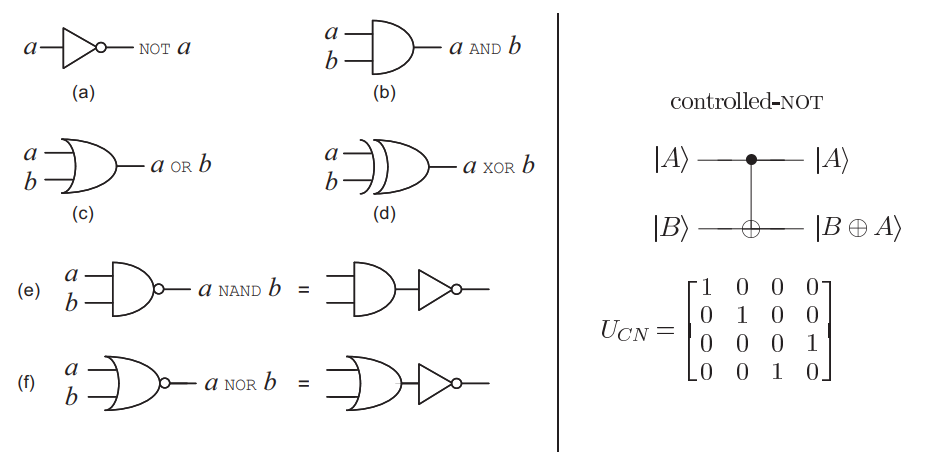
\includegraphics[scale=0.35]{FiveQ.png}}
        \end{minipage}\\
        \vspace{0.3cm}
        \footnotesize{\textbf{Рисунок 5} Слева расположены некоторые стандартные одно- и многоразрядные вентили, в то время как справа находится прототип
        многоразрядного кубитного вентиля, управляемый-NOT. Матричное представление управляемого-NOT, $U_{CN}$ , записывается
        относительно амплитуд для $\vert00\rangle,~\vert01\rangle,~\vert10\rangle$ и $\vert11\rangle$, в таком порядке.}
    \end{flushleft}
    \normalsize{
        Прототипным многокубитным квантовым логическим элементом является элемент controlled-NOT или CNOT.
        Этот элемент управления имеет два входных кубита, известных как \emph{управляющий} кубит и \emph{целевой} кубит соответственно. Схемное представление CNOT показано в правом верхнем углу рисунка 5;
        верхняя строка представляет управляющий кубит, в то время как нижняя строка представляет целевой кубит. Действие вентиля может быть описано следующим образом. Если управляющий кубит установлен в
        0, то целевой кубит остается в покое. Если управляющий кубит установлен в 1, то целевой кубит изменяется. В уравнениях:
        \begin{equation}
            \begin{split}
                \vert00\rangle\rightarrow \vert00\rangle;~\vert01\rangle\rightarrow\vert01\rangle; \\
                \vert10\rangle\rightarrow\vert11\rangle;~\vert11\rangle\rightarrow\vert10\rangle.
            \end{split}
        \end{equation}
        Другой способ описания CNOT "--- это обобщение классического элемента XOR, поскольку
        действие элемента может быть представлено как $\vert A,~B\rangle\rightarrow\vert A,~B\oplus A\rangle$, где $\oplus$ "--- сложение по модулю 2, что именно и делает XOR, 
        то есть над контрольным и целевым кубитами проводится XOR, и результат сохраняется в целевой кубит.

        Еще одним способом описания действия CNOT является предоставление матричного представления, как показано в правом нижнем углу рисунка 5. Вы можете легко убедиться, что первый 
        столбец $U_{CN}$ описывает преобразование, которое происходит с $\vert00\rangle$, и аналогично для
        других вычислительных базовых состояний, $\vert01\rangle$, $\vert10\rangle$, и $\vert11\rangle$. 
        Что касается случая с одним кубитом, то требование сохранения вероятности выражается в том факте, что $U_{CN}$ является унитарной
        матрицей, то есть $U_{CN}^{\dagger}U_{CN}=I$.

        Мы заметили, что CNOT можно рассматривать как тип обобщенного элемента XOR. Могут
        ли другие классические элементы, такие как NAND или обычный элемент XOR пониматься как унитарные
        элементы в смысле, аналогичном тому, как квантовый элемент NOT представляет классический
        элемент NOT? Оказывается, это невозможно. Причина в том, что элементы XOR и NAND
        по существу необратимы. Например, учитывая выходные данные $A\oplus B$ из
        элемента XOR, невозможно определить, какими были входные данные A и B; существует
        безвозвратная потеря информации, связанная с необратимым действием элемента XOR.
        С другой стороны, унитарные квантовые вентили всегда обратимы, поскольку инверсия
        унитарной матрицы также является унитарной матрицей, и, таким образом, квантовый вентиль всегда может быть инвертирован
        другим квантовым вентилем. Понимание того, как использовать классическую логику в этом
        обратимом смысле, станет решающим шагом в понимании того, как использовать мощь квантовой механики для вычислений.

        Конечно, есть много интересных квантовых вентилей, отличных от контролируемых-NOT.
        Однако в некотором смысле элементы с управляемым-NOT и однокубитным вентилем являются прототипами для всех
        других элементов из-за следующего замечательного результата универсальности: любой
        логический элемент с несколькими кубитами может быть составлен из элементов CNOT и одиночных кубитов.
    }\\
    \section*{Измерения в базах, отличных от расчетной базы}
    \normalsize{
        Мы описали квантовые измерения одного кубита в состоянии $\alpha\vert0\rangle+\beta\vert1\rangle$ как
        дающие результат 0 или 1 и оставляющие кубит в соответствующем состоянии $\vert0\rangle$ или $\vert1\rangle$ 
        с соответствующими вероятностями $\vert\alpha\vert^2$ и $\vert\beta\vert^2$. На самом деле, квантовая механика допускает несколько
        большую универсальность в классе измерений, которые могут быть выполнены, хотя, конечно, далеко не настолько, чтобы восстановить $\alpha$ и $\beta$ из одного измерения!

        Обратите внимание, что состояния $\vert0\rangle$ и $\vert1\rangle$ представляют собой лишь один из многих возможных вариантов базовых
        состояний для кубита. Другим возможным выбором является набор $\vert+\rangle\equiv(\vert0\rangle+\vert1\rangle)/\sqrt2$ и $\vert-\rangle\equiv(\vert0\rangle-\vert1\rangle)/\sqrt2$.
        Произвольное состояние $\vert\psi\rangle=\alpha\vert0\rangle+\beta\vert1\rangle$ может быть повторно выражено в терминах состояний $\vert+\rangle$ и $vert-\rangle$:
        \begin{equation}
            \begin{split}
                \vert\psi\rangle=\alpha\vert0\rangle+\beta\vert1\rangle=\alpha\frac{\vert+\rangle+\vert-\rangle}{\sqrt2}+\\\beta\frac{\vert+\rangle-\vert-\rangle}{\sqrt2}=\frac{\alpha+\beta}{\sqrt2}\vert+\rangle+\frac{\alpha-\beta}{\sqrt2}\vert-\rangle.
            \end{split}
        \end{equation}
        Оказывается, что можно рассматривать состояния $\vert+\rangle$ и $\vert-\rangle$ так, как если бы они были вычислительными базисными состояниями, и измерять относительно этого нового базиса. 
        Естественно, измерение по отношению к базису $\vert+\rangle$, $\vert-\rangle$ приводит к результату <<$+$>> с вероятностью $\vert\alpha+\beta\vert^2/2$ 
        и к результату <<$-$>> с вероятностью $\vert\alpha-\beta\vert^2/2$, с соответствующими состояниями $\vert+\rangle$ и $\vert-\rangle$ после измерения.
        
        В более общем плане, учитывая любые базисные состояния $\vert a\rangle$ и $\vert b\rangle$ для кубита, можно выразить
        произвольное состояние как линейную комбинацию $\alpha\vert a\rangle + \beta\vert b \rangle$  этих состояний.
        Кроме того, при условии, что состояния \emph{ортонормированы}, можно выполнить измерение относительно
        базиса $\vert a\rangle,~\vert b\rangle$, получая результат $a$ с вероятностью $\alpha^2$ и $b$ с вероятностью $\beta^2$.
        Ограничение ортонормированности необходимо для того, чтобы $\vert\alpha\vert^2+\vert\beta\vert^2=1$, как мы и ожидаем для
        вероятностей. Аналогичным образом в принципе возможно измерить квантовую систему
        из многих кубитов относительно произвольного ортонормированного базиса.
    }\\
    \section*{Квантовые схемы}
    \normalsize{
        Давайте рассмотрим чуть более подробно элементы квантовой схемы. Простая квантовая схема, содержащая три квантовых
        элемента, показана на рис. 6. Схема должна считываться слева направо. 
        Каждая линия в схеме представляет собой провод в квантовой схеме. Этот провод не обязательно
        соответствует физическому проводу; вместо этого он может соответствовать течению времени или, возможно, 
        физической частице, такой как фотон "--- частица света, перемещающаяся из одного места
        в другое в пространстве. Принято считать, что состояние, входящее в схему
        является базовым вычислительным состоянием, обычно состоянием, состоящим из всех $\vert0\rangle$. Это правило
        часто нарушается в литературе по квантовым вычислениям и квантовой информации, но
        считается вежливым информировать читателя, что это имеет место.

        Схема на рис. 6 выполняет простую, но полезную задачу "--- она меняет местами состояния
        двух кубитов. Чтобы увидеть, что эта схема выполняет операцию \emph{swap}, обратите внимание, что
        последовательность элементов имеет следующую последовательность воздействий на вычислительное базовое состояние $\vert a,b\rangle$,
        \begin{equation}
            \begin{split}
                \vert a,b \rangle \longrightarrow \vert a,a\oplus b\rangle\\
                \longrightarrow \vert a\oplus(a\oplus b),a\oplus b\rangle = \vert b,a\oplus b\rangle\\
                \longrightarrow \vert b,(a\oplus b)\oplus b \rangle=\vert b,a\rangle,
            \end{split}
        \end{equation}
        где все сложения производятся по модулю 2. Таким образом, эффект схемы заключается в обмене состояниями двух кубитов.
    }\\
    \begin{flushleft}
        \begin{minipage}{0.3\textwidth}{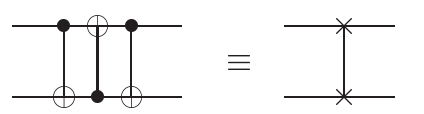
\includegraphics[scale=0.78]{cir.png}}
        \end{minipage}\\
        \vspace{0.3cm}
        \footnotesize{\textbf{Рисунок 6} Схема, заменяющая два кубита, и эквивалентное схематическое обозначение для этой распространенной и полезной схемы.}
    \end{flushleft}
    \normalsize{
        В классических схемах разрешено несколько функций, которые обычно не присутствуют в
        квантовых схемах. Прежде всего, мы не допускаем <<петель>>, то есть обратной связи от одной части
        квантовой схемы к другой; мы говорим, что схема ациклическая. Во-вторых, классические схемы позволяют
        <<соединять>> провода вместе, операция, известная как FANIN, при этом результирующий одиночный провод
        содержит побитовое OR входов. Очевидно, что эта операция необратима и
        , следовательно, не является унитарной, поэтому мы не допускаем FANIN в наших квантовых схемах. В-третьих, обратное
        операция FANOUT, при которой создается несколько копий бита, также не допускается в
        квантовых схемах. Фактически, оказывается, что квантовая механика запрещает копирование
        кубита, что делает операцию FANOUT невозможной!

        По мере продвижения мы будем вводить новые квантовые элементы по мере необходимости. На этом этапе удобно ввести еще одно соглашение о квантовых схемах. Это соглашение
        проиллюстрировано на рис. 7. Предположим, что $U$ "--- любая унитарная матрица, действующая на некоторое число n
        кубитов, поэтому $U$ можно рассматривать как квантовый вентиль на этих кубитах. Затем мы можем определить
        элемент controlled-$U$, который является естественным продолжением элемента controlled-NOT. Такой вентиль
        имеет один контрольный кубит, обозначенный линией с черной точкой, и n целевых кубитов,
        обозначается буквой $U$ в рамке. Если контрольный кубит установлен в 0, то с
        целевыми кубитами ничего не происходит. Если контрольный кубит установлен в 1, то элемент $U$ применяется к целевым кубитам.
        Прототипическим примером элемента controlled-$U$ является элемент controlled-NOT, который представляет
        собой элемент controlled-$U$ с $U = X$, как показано на рисунке 8.
    }\\
    \begin{center}
        \begin{minipage}{0.3\textwidth}{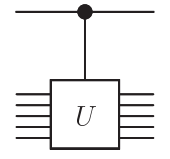
\includegraphics[scale=0.9]{cug.png}}
        \end{minipage}\\
        \vspace{0.3cm}
        \footnotesize{\textbf{Рисунок 7} controlled-$U$ вентиль.}
    \end{center}
    \begin{flushleft}
        \begin{minipage}{0.3\textwidth}{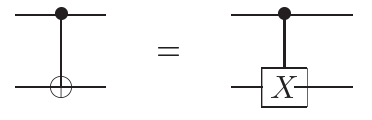
\includegraphics[scale=0.9]{cnotg.png}}
        \end{minipage}\\
        \vspace{0.3cm}
        \centering{\footnotesize{\textbf{Рисунок 8} Два разных представления controlled-NOT вентиля}}
    \end{flushleft}
    \normalsize{
        Другой важной операцией является измерение, которое мы обозначаем символом <<$M$>>, как показано на рисунке 9. Как описано ранее, эта операция преобразует
        состояние одиночного кубита $\vert\psi\rangle = \alpha\vert0\rangle + \beta\vert1\rangle$ в вероятностный классический бит $M$ (отличающийся от кубита
        тем, что он представлен в виде двухлинейного провода), который равен 0 с вероятностью $\vert\alpha\vert^2$ и 1 с вероятностью $\vert\beta\vert^2$.
    }\\
    \begin{center}
        \begin{minipage}{0.3\textwidth}{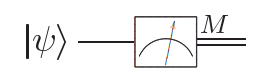
\includegraphics[scale=0.9]{Mg.png}}
        \end{minipage}\\
        \vspace{0.3cm}
        \centering{\footnotesize{\textbf{Рисунок 9} Символ квантовой схемы для измерения.}}
    \end{center}
    \normalsize{
        Квантовые схемы полезны в качестве моделей всех квантовых процессов, включая коммуникацию и даже квантовый шум. Ниже приведены несколько простых
        примеров, иллюстрирующих это.
    }\\
    \section*{Кубит копирует схему?}
    \normalsize{
        Элемент CNOT полезен для демонстрации одного особенно фундаментального свойства
        квантовой информации. Рассмотрим задачу копирования классического бита. Это может быть сделано
        с помощью классического элемента CNOT, который принимает бит для копирования (в некотором неизвестном состоянии $x$)
        и бит <<блокнота>>, инициализированный нулем, как показано на рисунке 10. На выходе получается два
        бита, находящиеся в одном и том же состоянии $x$.

        Предположим, мы пытаемся скопировать кубит в неизвестном состоянии $\vert\psi\rangle=a \vert0\rangle+b \vert1\rangle$ таким же
        образом, используя элемент CNOT. Входное состояние двух кубитов может быть записано как
        \begin{equation}
            \big[a\vert0\rangle+b\vert1\rangle\big]\vert0\rangle=a\vert00\rangle+b\vert10\rangle,
        \end{equation}
        Функция CNOT состоит в том, чтобы применить отрицание ко второму кубиту, когда первый равен 1, и, таким образом, 
        на выходе получается просто $a\vert00\rangle+b\vert11\rangle$. Успешно ли мы скопировали $\vert\psi\rangle$? 
        То есть, создали ли мы состояние $\vert\psi\rangle\vert\psi\rangle$? В случае, когда $\vert\psi\rangle=\vert0\rangle$ или $\vert\psi\rangle=\vert1\rangle$, это действительно то, что делает 
        схема; можно использовать квантовые схемы для копирования классической информации, закодированной как $\vert0\rangle$ или $\vert1\rangle$.  Однако для общего состояния $\vert\psi\rangle$ мы видим, что
        \begin{equation}
            \vert\psi\rangle\vert\psi\rangle=a^2\vert00\rangle+ab\vert01\rangle+ab\vert10\rangle+b^2\vert11\rangle.
        \end{equation}
    }\\
    \begin{flushleft}
        \begin{minipage}{0.3\textwidth}{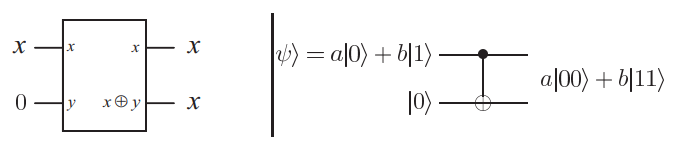
\includegraphics[scale=0.45]{qcopy.png}}
        \end{minipage}\\
        \vspace{0.3cm}
        \centering{\footnotesize{\textbf{Рисунок 10} Классические и квантовые схемы для <<копирования>> неизвестного бита или кубита.}}
    \end{flushleft}
    \normalsize{
        Сравнивая с $a\vert00\rangle+b\vert11\rangle$, мы видим, что, если $ab = 0$, описанная выше <<схема копирования>> 
        \emph{не} копирует входное квантовое состояние. На самом деле, оказывается невозможным создать копию
        неизвестного квантового состояния. Это свойство, заключающееся в том, что кубиты не могут быть скопированы, известно
        как теорема о недопустимости клонирования, и это одно из главных отличий квантовой
        информации от классической.

        Существует другой способ взглянуть на сбой схемы на рис. 10, основанный на
        интуиции, что кубит каким"=то образом содержит <<скрытую>> информацию, недоступную
        непосредственно измерению. Рассмотрим, что происходит, когда мы измеряем один из кубитов состояния $a\vert00\rangle+b\vert11\rangle$. 
        Как описано ранее, мы получаем либо $0$, либо $1$ с вероятностями $\vert a\vert^2$ и $\vert b\vert^2$. Однако, как только один кубит измерен, состояние другого кубита полностью
        определено, и никакой дополнительной информации об $a$ и $b$ получить невозможно. В этом смысле,
        дополнительная скрытая информация, содержащаяся в исходном кубите $\vert\psi\rangle$, была потеряна при первом измерении и не может быть восстановлена. Однако если кубит был скопирован, то состояние
        другого кубита все равно должно содержать часть этой скрытой информации. Следовательно, копия не могла быть создана.
    }\\
    \section*{Пример: Состояния Белла} 
    \normalsize{
        Давайте рассмотрим немного более сложную схему, показанную на рис. 11, которая имеет
        элемент Адамара, за которым следует CNOT, преобразущую четыре вычислительных базовых состояния
        в соответствии с приведенной таблицей. В качестве явного примера, элемент Адамара принимает входные данные от $\vert00\rangle$ до $(\vert0\rangle+\vert1\rangle)\vert0\rangle/\sqrt2$, и затем CNOT выдает выходное состояние $(\vert00\rangle+\vert11\rangle)/\sqrt2$.
        Обратите внимание, как это работает: во-первых, преобразование Адамара помещает верхний кубит в суперпозицию;
        затем это действует как управляющий вход для CNOT, и цель инвертируется только тогда, когда
        значение элемента управления равно 1. Выходные состояния
        \begin{equation}
            \vert\beta_{00}\rangle=\frac{\vert00\rangle+\vert11\rangle}{\sqrt2};
        \end{equation}
        \begin{equation}
            \vert\beta_{01}\rangle=\frac{\vert01\rangle+\vert10\rangle}{\sqrt2};
        \end{equation}
        \begin{equation}
            \vert\beta_{10}\rangle=\frac{\vert00\rangle-\vert11\rangle}{\sqrt2};
        \end{equation}
        \begin{equation}
            \vert\beta_{11}\rangle=\frac{\vert01\rangle-\vert10\rangle}{\sqrt2}.
        \end{equation}
        известны как \emph{состояния Белла}, или иногда \emph{состояния} EPR или \emph{пары} EPR, в честь некоторых
        людей "--- Белла, Эйнштейна, Подольского и Розена, "--- которые первыми указали на странные
        свойства подобных состояний. Мнемоническое обозначение $\vert\beta_{00}\rangle,~\vert\beta_{01}\rangle,~\vert\beta_{10}\rangle,~\vert\beta_{11}\rangle$ может пониматься из равенств
        \begin{equation}
            \vert\beta_{\text{xy}}\rangle\equiv\frac{\vert0,\text{y}\rangle+(-1)^{\text{x}}\vert1,\bar{\text{y}}\rangle}{\sqrt2},
        \end{equation}
        где $\bar{y}$ "--- отрицание $y$.
    }\\
    \begin{flushleft}
        \begin{minipage}{0.3\textwidth}{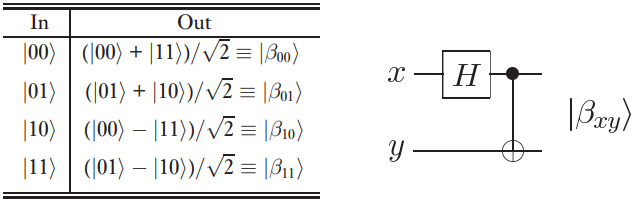
\includegraphics[scale=0.5]{bell.png}}
        \end{minipage}\\
        \vspace{0.3cm}
        \centering{\footnotesize{\textbf{Рисунок 11} Квантовая схема для создания состояний Белла и ее входно–выходная квантовая <<таблица истинности>>.}}
    \end{flushleft}
    \section*{Пример: квантовая телепортация}
    \normalsize{
        Теперь мы применим методы, описанные на последних нескольких страницах, чтобы понять нечто нетривиальное, удивительное и очень забавное "--- квантовую телепортацию! Квантовая телепортация "--- это
        метод перемещения квантовых состояний даже при отсутствии квантового канала связи, связывающего отправителя квантового состояния с получателем.
        Вот как работает квантовая телепортация. Алиса и Боб познакомились давным-давно, но сейчас живут
        далеко друг от друга. Находясь вместе, они генерировали EPR-пару, каждый из них брал по одному кубиту из EPR-пары, 
        когда они разделялись. Много лет спустя Боб скрывается, и миссия Алисы "--- 
        доставить кубит $\vert\psi\rangle$ Бобу. Она не знает состояния
        кубита и, более того, может отправлять Бобу только \emph{классическую} информацию. Должна ли Алиса взяться за эту миссию?

        Интуитивно, для Алисы все выглядит довольно плохо. Она не знает состояния $\vert\psi\rangle$
        кубита, который она должна отправить Бобу, и законы квантовой механики не позволяют ей
        определить состояние, когда в ее распоряжении есть только одна копия $\vert\psi\rangle$. Что еще
        хуже, даже если бы она знала состояние $\vert\psi\rangle$, для его точного описания требуется бесконечное количество
        классической информации, поскольку $\vert\psi\rangle$ принимает значения в непрерывном пространстве. Так что даже если бы она
        знала $\vert\psi\rangle$, Алисе потребовалась бы вечность, чтобы описать Бобу это состояние. 
        К счастью для Алисы, квантовая телепортация "--- это способ использования
        запутанной пары EPR для отправки $\vert\psi\rangle$ Бобу с небольшими накладными расходами по сравнению с \emph{классической}
        коммуникацией.

        В общих чертах этапы решения следующие: Алиса взаимодействует с кубитом $\vert\psi\rangle$ со
        своей половиной EPR пары, а затем измеряет два имеющихся в ее распоряжении кубита, получая
        один из четырех возможных классических результатов: 00, 01, 10 и 11. Она отправляет эту информацию
        Бобу. В зависимости от классического сообщения Алисы Боб выполняет одну из четырех операций со своей
        половиной EPR пары. Удивительно, но, сделав это, он может восстановить исходное состояние $\vert\psi\rangle!$

        Квантовая схема, показанная на рис. 12, дает более точное описание квантовой
        телепортации. Состояние, подлежащее телепортации "--- $\vert\psi\rangle=\alpha\vert0\rangle+\beta\vert1\rangle$ где $\alpha$ и $\beta$ "--- неизвестные
        амплитуды. Состояние $\vert\psi_{0}\rangle$, которое схема получает на вход, равно
        \begin{equation}
            \vert\psi{0}\rangle = \vert\psi\rangle\vert\beta_{00}\rangle=
        \end{equation}
    }\\
    \begin{flushleft}
        \begin{minipage}{0.3\textwidth}{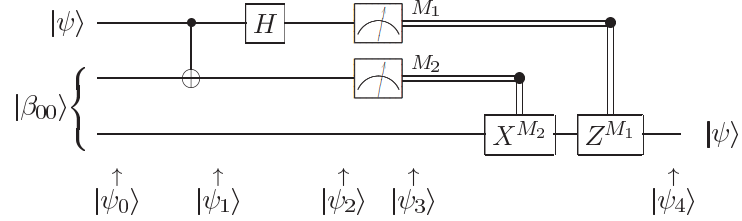
\includegraphics[scale=0.5]{tp.png}}
        \end{minipage}\\
        \vspace{0.3cm}
        \centering{\footnotesize{\textbf{Рисунок 12} Квантовая схема для телепортации кубита. Две верхние строки представляют систему Алисы, в то время как нижняя
        строка "--- систему Боба. Счетчики представляют собой измерение, а двойные линии, выходящие из них, несут классические
        биты (напомним, что одиночные линии обозначают кубиты).}}
    \end{flushleft}
    \normalsize{
        \begin{equation}
            =\frac{1}{\sqrt2}\big[\alpha\vert0\rangle(\vert00\rangle+\vert11\rangle)+\beta\vert1\rangle(\vert00\rangle+\vert11\rangle)\big],
        \end{equation}
        где мы используем соглашение о том, что первые два кубита (слева) принадлежат Алисе, а
        третий кубит "--- Бобу. Как мы объясняли ранее, второй кубит Алисы и кубит Боба
        начинаются в состоянии EPR. Алиса отправляет свои кубиты через CNOT, получая
        \begin{equation}
            \vert\psi_{1}\rangle=\frac{1}{\sqrt2}\big[\alpha\vert0\rangle(\vert00\rangle+\vert11\rangle)+\beta\vert1\rangle(\vert10\rangle+\vert01\rangle)\big].
        \end{equation}
        Затем она отправляет первый кубит через вентиль Адамара, получая
        \begin{equation}
            \begin{split}
                \vert\psi_{2}\rangle=\frac{1}{2}\big[\alpha(\vert0\rangle+\vert1\rangle)(\vert00\rangle+\vert11\rangle)+\\\beta(\vert0\rangle-\vert1\rangle)(\vert10\rangle+\vert01\rangle)\big].
            \end{split}
        \end{equation}
        Это состояние может быть переписано следующим образом, просто перегруппировав элементы:
        \begin{equation}
            \begin{split}
                \vert\psi_{2}\rangle=\frac{1}{2}\big[\vert00\rangle(\alpha\vert0\rangle+\beta\vert1\rangle)+\vert01\rangle(\alpha\vert1\rangle+\beta\vert0\rangle)\\
                +\vert10\rangle(\alpha\vert0\rangle-\beta\vert1\rangle)+\vert11\rangle(\alpha\vert1\rangle-\beta\vert0\rangle)\big].            \end{split}
        \end{equation}
        Это выражение, естественно, распадается на четыре члена. Первый член содержит кубиты Алисы
        в состоянии $\vert00\rangle$, а кубит Боба "--- в состоянии $\alpha\vert0\rangle+\beta\vert1\rangle$, которое является исходным состоянием
        $\vert\psi\rangle$.  Аналогично, из предыдущего выражения мы можем считать состояние Боба после измерения, учитывая результат измерения Алисы:
        \begin{equation}
            00\longmapsto \vert\psi_{3}(00)\rangle\equiv\big[\alpha\vert0\rangle+\beta\vert1\rangle\big]
        \end{equation}
        \begin{equation}
            01\longmapsto \vert\psi_{3}(01)\rangle\equiv\big[\alpha\vert1\rangle+\beta\vert0\rangle\big]
        \end{equation}
        \begin{equation}
            10\longmapsto \vert\psi_{3}(10)\rangle\equiv\big[\alpha\vert0\rangle-\beta\vert1\rangle\big]
        \end{equation}
        \begin{equation}
            11\longmapsto \vert\psi_{3}(11)\rangle\equiv\big[\alpha\vert1\rangle-\beta\vert0\rangle\big].
        \end{equation}
        В зависимости от результата измерения Алисы кубит Боба окажется в одном из этих
        четырех возможных состояний. Конечно, чтобы узнать, в каком состоянии он находится, Бобу необходимо сообщить результат
        измерения Алисы "--- позже мы покажем, что именно этот факт не позволяет использовать телепортацию для передачи информации быстрее света.
        Как только Боб узнает результат измерения, он может <<исправить>> свое состояние, восстановив $\vert\psi\rangle$, применив соответствующий
        квантовый вентиль. Например, в случае, когда измерение дает результат 00, Бобу ничего не нужно делать. Если значение равно 01, то Боб может исправить свое состояние, применив
        элемент X. Если значение равно 10, то Боб может исправить свое состояние, применив элемент Z. Если значение равно 11, то Боб может исправить свое состояние, применив сначала элемент X, а
        затем Z. В итоге Бобу придется применить $Z^{M_1}X^{M_2}$ (обратите внимание, как
        на схемах время идет слева направо, но в матричных произведениях термины справа
        появляются первыми) к своему кубиту, и он восстановит состояние $\vert\psi\rangle$.

        Во-первых, разве телепортация не позволяет передавать квантовые состояния быстрее
        света? Это было бы довольно странно, поскольку теория относительности подразумевает, что
        передача информации со скоростью, превышающей скорость света, может быть использована для отправки информации назад во времени.
        К счастью, квантовая телепортация не обеспечивает связь быстрее света,
        потому что для завершения телепортации Алиса должна передать результат своего измерения в
        Боб по классическому каналу связи. Без классической коммуникации телепортация вообще не передает никакой информации. 
        Классический канал ограничен скоростью света, из чего следует, что квантовая телепортация
        не может быть осуществлена быстрее скорости света, разрешая кажущийся парадокс.

        Вторая загадка, связанная с телепортацией, заключается в том, что она, по-видимому, создает копию телепортируемого квантового состояния, что явно нарушает теорему о недопустимости клонирования, обсуждаемую 
        ранее. Это нарушение является лишь иллюзорным, поскольку после процесса телепортации только
        целевой кубит остается в состоянии $\vert\psi\rangle$, а исходный кубит данных оказывается в одном из базовых
        вычислительных состояний $\vert0\rangle$ или $\vert1\rangle$, в зависимости от результата измерения в первом кубите.

        Чему мы можем научиться из квантовой телепортации? Довольно многому! Это гораздо больше, чем
        просто изящный трюк, который можно проделать с квантовыми состояниями. Квантовая телепортация подчеркивает
        взаимозаменяемость различных ресурсов в квантовой механике, показывая, что общая
        пара EPR вместе с двумя классическими битами связи представляет собой ресурс, по меньшей мере
        равный одному кубиту связи. Квантовые вычисления и квантовая информация
        выявили множество методов обмена ресурсами, многие из которых основаны на квантовой
        телепортации.

        Телепортация может быть использована для создания квантовых вентилей, устойчивых к воздействию шума, также телепортация тесно связана со свойствами квантовых
        кодов, исправляющих ошибки.
    }\\
    \section*{Оптический фотонный квантовый компьютер}
    \normalsize{
        Привлекательной физической системой для представления квантового бита является оптический фотон. Фотоны "--- это частицы без заряда, и они не очень сильно взаимодействуют друг с другом или даже
        с большей частью материи. Их можно направлять на большие расстояния с малыми потерями в оптических волокнах,
        эффективно задерживать с помощью фазовращателей и легко комбинировать с помощью светоделителей. Фотоны
        демонстрируют характерные квантовые явления, такие как интерференция, возникающая в экспериментах с двумя щелями. Более того, в принципе, фотоны можно заставить взаимодействовать друг с другом.
        С этим идеальным сценарием связаны проблемы; тем не менее,
        как мы увидим в этом разделе, из изучения компонентов, архитектуры и недостатков оптического фотонного квантового информационного процессора можно многому научиться.

        Давайте начнем с рассмотрения того, что такое одиночные фотоны, как они могут представлять квантовые
        состояния и экспериментальные компоненты, полезные для манипулирования фотонами. Описано классическое
        поведение фазовращателей, расщепителей луча и нелинейно-оптических сред Керра.нергия в электромагнитном резонаторе квантуется
        в единицах $\hbar\omega$. Каждый такой квант называется фотоном. Полость может 
        содержать суперпозицию нуля или одного фотона, состояние которого можно было бы выразить как кубит
        $c_0\vert0\rangle+c_1\vert1\rangle$, но мы сделаем кое-что другое. Давайте рассмотрим две полости,
        суммарная энергия которых равна $\hbar\omega$, и примем два состояния кубита за то, находится ли фотон в одной полости $(\vert01\rangle$) или в другой $(\vert10\rangle)$. 
        Таким образом, физическое состояние суперпозиции было
        бы записано как $c_0\vert01\rangle+c_1\vert10\rangle$; мы будем называть это представление \emph{двойным рельсовым (dual-rail)}. 
        Обратите внимание, что мы сосредоточимся на одиночных фотонах, распространяющихся в виде волнового пакета в свободном пространстве, а не
        внутри полости; можно представить это как наличие полости, движущейся вместе с волновым пакетом. Таким образом, каждая полость в нашем состоянии кубита будет соответствовать другому пространственному режиму.

        Одна из схем генерации одиночных фотонов в лаборатории заключается в ослаблении мощности
        лазера. Лазер выводит состояние, известное как когерентное состояние, $\vert\alpha\rangle$, определяемое как
        \begin{equation}
            \vert\alpha\rangle=e^{-\vert\alpha\vert^2/2}\sum_{n = 0}^{\infty}  \frac{\alpha^n}{\sqrt{n!}}\vert n\rangle,
        \end{equation}
        где $\vert n\rangle$ "--- собственное состояние энергии n"=фотонов. Это состояние, которое было предметом
        тщательного изучения в области квантовой оптики, обладает многими прекрасными свойствами, которые мы
        не будем здесь описывать. Достаточно просто понять, что когерентные состояния естественным
        образом излучаются управляемыми генераторами, такими как лазер, при накачке выше порога генерации.
        Обратите внимание, что средняя энергия равна
        \begin{equation}
            \langle\alpha\vert n\vert\alpha\rangle=\vert\alpha\vert^2.
        \end{equation}
        При ослаблении когерентное состояние просто
        становится более слабым когерентным состоянием, и с высокой вероятностью можно сделать так, чтобы в слабом когерентном состоянии был только один фотон.

        Например, для $\alpha=\sqrt{0.1}$, мы получаем состояние $\sqrt{0.90}\vert0\rangle+\sqrt{0.09}\vert1\rangle+\sqrt{0.002}\vert2\rangle+\ldots$.
        Таким образом, если свет когда"=либо проходит через аттенюатор, человек знает, что это одиночный фотон с
        вероятностью более 95\%; таким образом, вероятность отказа составляет 5\%. Обратите также внимание, что в 90\%
        случаев фотоны вообще не проходят; таким образом, этот источник имеет скорость 0,1 фотона в единицу
        времени. Наконец, этот источник не указывает (посредством некоторого классического считывания),
        был ли выведен фотон или нет; два из этих источников не могут быть синхронизированы.

        Лучшей синхронности можно достичь с помощью параметрического понижающего преобразования. Это включает
        в себя отправку фотонов частоты $\omega_0$ в нелинейно"=оптическую среду, такую как $KH_2PO_4$, для
        генерации пар фотонов на частотах $\omega_1 + \omega_2 = \omega_0$. Импульс также сохраняется, так что 
        $\vec{k_1}+\vec{k_2}=\vec{k_3}$, так что когда (деструктивно) обнаруживается один фотон $\omega_2$, то 
        известно, что фотон $\omega_1$ существует (рис. 13).  Связывая это с вентилем, который открывается
        только при обнаружении одного фотона (в отличие от двух или более), и соответствующим образом
        задерживая выходные сигналы нескольких источников понижающего преобразования, можно, в принципе, получить
        множество одиночных фотонов, распространяющихся во времени синхронно, в пределах временного разрешения
        детектора и вентиля. 

        Одиночные фотоны могут быть обнаружены с высокой квантовой эффективностью в широком диапазоне
        длин волн с использованием различных технологий. Для наших целей наиболее важной характеристикой детектора является его способность с высокой вероятностью определять, существует ли
        ноль или один фотон в определенном пространственном режиме. Для представления с двумя рельсами
        это приводит к проективному измерению в вычислительном базисе. На практике несовершенства снижают вероятность обнаружения одиночного фотона; \emph{квантовая эффективность} 
        $\eta (0 \leq \eta \leq 1)$ 
        фотоприемника "--- это вероятность того, что одиночный фотон, падающий
        на детектор, генерирует пару фотоносителей, которые вносят вклад в ток детектора. Другими
        важными характеристиками детектора являются его полоса пропускания (чувствительность ко времени), шум и
        <<количество темных пятен>>, которые являются фотоносителями, генерируемыми даже при отсутствии падающих фотонов.
    }\\
    \begin{flushleft}
        \begin{minipage}{0.3\textwidth}{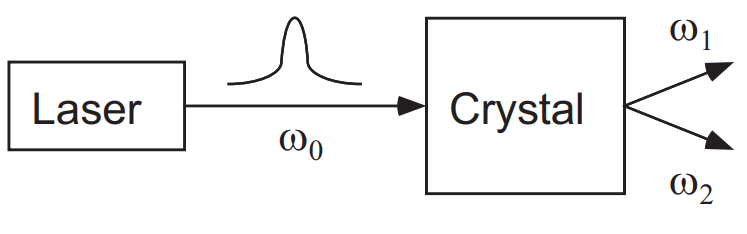
\includegraphics[scale=0.45]{lsqr.png}}
        \end{minipage}\\
        \vspace{0.3cm}
        \centering{\footnotesize{\textbf{Рисунок 13} Параметрическая схема понижающего преобразования для генерации одиночных фотонов.}}
    \end{flushleft}
    \normalsize{
        Тремя наиболее доступными в экспериментальном плане устройствами для манипулирования состояниями фотонов являются
        зеркала, фазовращатели и расщепители луча. Зеркала с высокой отражательной способностью отражают фотоны и
        изменяют направление их распространения в пространстве. Зеркала с потерями в 0,01\% не являются чем"=то необычным.
        Мы будем считать это само собой разумеющимся в нашем сценарии. Фазовращатель "--- это не что
        иное, как пластинка прозрачной среды с показателем преломления $n$, отличным от показателя преломления свободного
        пространства $n_0$; например, обычное боросиликатное стекло имеет $n\approx 1,5n_0$ на оптических длинах волн.
        Распространение в такой среде на расстояние $L$ изменяет фазу фотона на величину $e^{ikL}$,
        где $k = n\omega/c_0$, а $c_0$ "--- скорость света в вакууме. Таким образом, фотон, распространяющийся
        через фазовращатель, будет испытывать фазовый сдвиг $e^{i(n-n_0)L\omega/c_0}$ по сравнению с фотоном, 
        проходящим то же расстояние через свободное пространство.

        Другой полезный компонент, светоделитель, представляет собой не что иное, как частично посеребренный
        кусок стекла, который отражает долю $R$ падающего света и пропускает $1-R$. В
        лабораторных условиях светоделитель обычно изготавливается из двух призм,
        между которыми помещен тонкий металлический слой, схематически изображенный, как показано на рисунке 14. Удобно
        определить \emph{угол} $\theta$ светоделителя как $\cos{\theta} = R$; обратите внимание, что угол параметризует
        величину частичного отражения и не обязательно имеет какое-либо отношение к
        физической ориентации светоделителя. Два входа и два выхода этого устройства
        связаны между собой как
        \begin{equation}
            a_{out}=a_{in}\cos{\theta}+b_{in}\sin{\theta}
        \end{equation}
        \begin{equation}
            b_{out}=-a_{in}\sin{\theta}+b_{in}\cos{\theta},
        \end{equation}
        где классически мы рассматриваем $a$ и $b$ как электромагнитные поля излучения на
        двух портах. Обратите внимание, что в этом определении мы выбрали нестандартное соглашение о фазе, удобное для наших целей. В частном случае светоделителя (50/50), $\theta=45^\circ$.
    }\\
    \begin{flushleft}
        \begin{minipage}{0.3\textwidth}{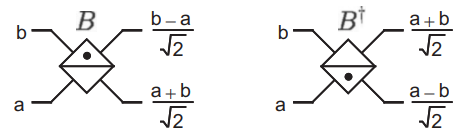
\includegraphics[scale=0.65]{bs5.png}}
        \end{minipage}\\
        \vspace{0.3cm}
        \centering{\footnotesize{\textbf{Рисунок 14} Схема оптического светоделителя, показывающая два входных порта, два выходных порта и фазовые
        соотношения для светоделителя 50/50 ($\theta = \frac{\pi}{4}$). Светоделитель справа является обратным по отношению к светоделителю слева
        (они различаются точкой, нарисованной внутри).}}
    \end{flushleft}
    \normalsize{
        Нелинейная оптика обеспечивает полезный компонент для этого: материал, показатель преломления которого n пропорционален общей интенсивности I проходящего через
        него света:
        \begin{equation}
            n(I)=n+n_2I.
        \end{equation}
        
        Произвольные унитарные преобразования могут быть применены к квантовой информации, закодированной одиночными фотонами в двухканальном представлении $c_0\vert01\rangle+c_1\vert10\rangle$, с использованием фазовращателей, расщепителей луча и нелинейно-оптических сред Керра. Как это работает, можно понять следующим образом, дав квантово-механическое гамильтоново описание каждого из этих устройств.

        Временная эволюция резонаторного режима электромагнитного излучения моделируется квантово-механически с помощью гармонического генератора.
        $\vert0\rangle$ "--- состояние вакуума, $\vert1\rangle=a^{\dagger}\vert0\rangle$ "--- состояние одиночного фотона, и в целом, $\vert n\rangle=\frac{a^{\dagger^n}}{\sqrt{n!}}\vert0\rangle$ "--- это n-фотонное состояние,где $a^{\dagger}$ "--- оператор создания режима. Эволюция свободного пространства описывается Гамильтонианом:
        \begin{equation}
            H=\hbar\omega a^{\dagger}a,
        \end{equation}
        и учитывая, что $\vert\psi(t)\rangle=e^{-iHt/\hbar}\vert \psi(0)\rangle=\sum_{n}^{} c_ne^{-in \omega t}\vert n\rangle$, мы находим, что состояние 
        $\vert\psi\rangle=c_0\vert0\rangle+c_1\vert1\rangle$ со временем изменяется к $\vert\psi(t)\rangle=c_0\vert0\rangle+c_1e^{-i\omega t}\vert1\rangle$.
        Обратите внимание, что представление с двумя рельсами удобно, поскольку свободная эволюция изменяет $\vert\phi\rangle=c_0\vert01\rangle+c_1\vert10\rangle$ только на общую фазу, которую невозможно обнаружить. Таким образом, для этого многообразия состояний эволюционный гамильтониан равен нулю.

        Фазовращатель. Фазовращатель $P$ действует точно так же, как обычная временная эволюция, но с другой скоростью и локализован только для режимов, проходящих через него. Это происходит потому, что свет замедляется в среде с большим показателем преломления; 
        в частности, для прохождения расстояния $L$ в среде с показателем преломления $n$ требуется на $\Delta\equiv(n-n_0)L/c_0$ больше времени, чем в вакууме. 
        Например, действие $P$ на вакуумное состояние состоит в том, чтобы ничего не делать: $P\vert0\rangle = \vert0\rangle$, но в однофотонном состоянии получается $P\vert1\rangle = e^{i\Delta}\vert1\rangle$. 

        P выполняет полезную логическую операцию в состоянии с двумя рельсами. Перевод фазовращателя в
        один режим замедляет его фазовую эволюцию по отношению к другому режиму, который проходит то же расстояние, но без прохождения через фазовращатель. Для состояний с двумя рельсами это преобразует 
        $c_0\vert01\rangle+c_1\vert10\rangle$ в $c_0e^{-i\Delta/2}\vert01\rangle+c_1e^{i\Delta/2}\vert10\rangle$, вплоть до несущественной общей фазы. Эта операция является не чем иным, как вращением,
        \begin{equation}
            R_{z}(\Delta)=e^{-iZ\Delta/2},
        \end{equation}
        где мы принимаем за логический ноль $\vert0_{L}\rangle=\vert01\rangle$ и единицу $\vert1_{L}\rangle=\vert10\rangle$, а $Z$ "--- оператор Паули. 
        Таким образом, можно думать о $P$ как о результате эволюции во времени в соответствии с Гамильтонианом
        \begin{equation}
            H=(n_0-n)Z,
        \end{equation}
        где $P=exp(-iHL/c_0).$

        Светоделитель. Аналогичное гамильтоново описание светоделителя также существует, но
        вместо того, чтобы мотивировать его феноменологически, давайте начнем с гамильтониана и покажем, как из него вытекает ожидаемое классическое поведение.
        Напомним, что светоделитель работает в двух режимах, которые мы опишем операторами создания (уничтожения) $a~(a^{\dagger})$ и $b~(b^{\dagger})$. Гамильтониан равен 
        \begin{equation}
            H_{bs}=i\theta(ab^{\dagger}-a^{\dagger}b),
        \end{equation}
        и светоделитель выполняет единую операцию
        \begin{equation}
            B=exp\big[\theta(a^{\dagger}b-ab^{\dagger})\big].
        \end{equation}
        Преобразования, произведенные $B$ над $a$ и $b$, которые позже окажутся полезными, оказались следующими 
        $BaB^{\dagger}=a\cos{\theta}+b\sin{\theta}$ и $BbB^{\dagger}=-a\sin{\theta}+b\cos{\theta}$.
        Мы проверяем эти соотношения, используя формулу Бейкера–Кэмпбелла–Хаусдорфа
        \begin{equation}
            e^{\lambda G}Ae^{-\lambda G}=\sum_{n = 0}^{\infty}  \frac{\lambda^n}{n!}C_n,
        \end{equation}
        где $\lambda$ "--- комплексное число, $A,~G,~C_n$ "--- операторы, и $C_n$ определяется рекурсивно как последовательность коммутаторов 
        $C_0=A,C_1=[G,C_0],C_2=[G,C_1],\ldots,C_n=[G,C_{n-1}].$ Поскольку из $[a,a^{\dagger}] = 1$ и $[b,b^{\dagger}]=1$ следует, что $[G,a]=-b$ и $[G,b]=a$ 
        для $G\equiv a^{\dagger}b-ab^{\dagger}$, мы получаем для разложения $BaB^{\dagger}$ коэффициенты ряда $C_0=a,C_1=[G,a]=-b,C_2=[G,C_1]=-a,C_3=[G,C_2]=-[G,C_0]=b$, что в общем случае 
        \begin{equation}
            C_{n~even} = i^na
        \end{equation}
        \begin{equation}
            C_{n~odd} = i^{n+1}b.
        \end{equation}
        Из этого прямо вытекает наш желаемый результат:
        \begin{equation}
            \begin{split}
                BaB^{\dagger}=e^{\theta G}ae^{-\theta G} \\
                = \sum_{n = 0}^{\infty} \frac{\theta^n}{n!}C_n \\
                = \sum_{n~even}^{}  \frac{(i\theta)^n}{n!}a+i \sum_{n~odd}^{} \frac{(i\theta)^n}{n!}b \\
                = a \cos{\theta} - b \sin{\theta}.
            \end{split}
        \end{equation}


        Это известно как оптический эффект Керра, и он проявляется (очень слабо) в
        таких обыденных материалах, как стекло и сахарная вода. В легированных стеклах $n_2$ колеблется от $10^{-14}$ до $10^{-7}$ $\text{см}^2/\text{Вт}$,
        а в полупроводниках "--- от $10^{-10}$ до $10^2$.
        Экспериментально соответствующее поведение заключается в том, что
        когда два пучка света равной интенсивности почти совместно распространяются через
        среду Керра, каждый пучок будет испытывать дополнительный фазовый сдвиг $e^{in_2IL\omega / c_0}$ по сравнению с тем, что
        происходит в случае с одним пучком. Это было бы идеально, если бы длина $L$ могла быть произвольной
        долго, но, к сожалению, это не удается, потому что большинство материалов Керра также обладают высокой поглощающей
        способностью или рассеивают свет не в желаемом пространственном режиме. Это основная причина, по которой однофотонный квантовый компьютер непрактичен.

        Однофотонное представление кубита привлекательно. Одиночные фотоны относительно
        просты в генерировании и измерении, а в представлении с двумя рельсами возможны произвольные
        операции с одним кубитом. К сожалению, взаимодействие фотонов затруднено "--- лучшие доступные нелинейные среды Керра очень слабы и не могут обеспечить перекрестную фазовую модуляцию
        $\pi$ между состояниями одиночных фотонов. На самом деле, поскольку нелинейный показатель преломления обычно
        получается при использовании среды вблизи оптического резонанса, всегда присутствует некоторое поглощение
        связанное с нелинейностью, и теоретически можно оценить, что при наилучшем таком
        расположении должно быть поглощено приблизительно 50 фотонов для каждого фотона, который испытывает $\pi$-перекрестную фазовую модуляцию. Это означает, что перспективы создания квантовых
        компьютеров из традиционных компонентов нелинейной оптики в лучшем случае невелики.

        Тем не менее, изучая этот оптический квантовый компьютер, мы получили некоторое
        ценное представление о природе архитектуры и системного проектирования квантового
        компьютера. Теперь мы можем видеть, как мог бы выглядеть настоящий квантовый компьютер в
        лаборатории (если бы для его создания были доступны только достаточно качественные компоненты), и
        поразительной особенностью является то, что он почти полностью построен из оптических интерферометров.
        В устройстве информация кодируется как в номере фотона, так и в фазе
        фотона, и для преобразования между этими двумя представлениями используются интерферометры.
        Хотя возможно сконструировать стабильные оптические интерферометры, если бы было выбрано альтернативное, массивное
        представление кубита, то быстро стало бы трудно создавать
        стабильные интерферометры из-за короткости типичных длин волн де Бройля.

        Исторически сложилось так, что классические оптические компьютеры когда-то считались многообещающей заменой электронным машинам, но в конечном счете они не оправдали ожиданий, когда не были открыты в достаточной степени нелинейные оптические материалы и когда их преимущества в скорости и параллелизме недостаточно перевешивали недостатки в выравнивании и мощности. С другой стороны, оптическая связь является жизненно важной областью; одной из причин этого является то, что на расстояниях более одного сантиметра энергия, необходимая для передачи бита с использованием фотона по волокну, меньше энергии, необходимой для зарядки обычного
        электронная линия передачи 50 Ом, покрывающая то же расстояние. Аналогичным образом, возможно, что оптические кубиты могут найти естественное применение при передаче квантовой информации, например, в квантовой криптографии, а не в вычислениях.
    }\\
    \section*{Физическая реализация}
    \normalsize{
    Каковы \emph{экспериментальные требования} для создания квантового компьютера? Элементарными единицами теории являются квантовые биты~--– двухуровневые квантовые системы.
    Чтобы реализовать квантовый компьютер, мы должны не только дать кубитам некоторое надежное физическое представление (в котором они сохраняют свои квантовые свойства), но
    и выбрать \emph{систему}, в которой их можно заставить эволюционировать по желанию. Кроме того, мы
    должны уметь подготавливать кубиты в некотором \emph{заданном} наборе начальных состояний и измерять
    конечное выходное состояние системы.

    Проблема экспериментальной реализации заключается в том, что эти основные требования часто могут
    быть выполнены лишь частично. Монета имеет два состояния и является хорошим битом, но плохим кубитом, потому что она не может оставаться в состоянии суперпозиции (<<орла>> и <<решки>>) очень долго.
    Одиночный ядерный спин может быть очень хорошим кубитом, потому что суперпозиции выравнивания
    с внешним магнитным полем или против него могут сохраняться долгое время~--– даже в течение нескольких дней. Но
    построить квантовый компьютер из ядерных спинов может быть трудно из-за проблемы в измерии ориентации отдельных ядер.
    
    Требования весьма противоречивы: квантовый компьютер должен быть
    хорошо \emph{изолирован}, чтобы сохранить свои квантовые свойства, но в то же время его кубиты
    должны быть \emph{доступны}, чтобы ими можно было манипулировать для выполнения вычислений и
    считывания результатов. Реализация должна обеспечивать тонкий баланс между
    этими ограничениями, так что актуальный вопрос заключается не в том, как построить квантовый компьютер,
    а скорее в том, насколько хороший квантовый компьютер может быть построен.
    }\\
    \section*{Квантовый компьютер} 
    \normalsize{
    Схема квантового компьютера представлена на рис. 13.
    По существу квантовый компьютер представляет собой \emph{регистр} из $n$ кубитов,
    управляемых внешними (классическими) сигналами. Квантовый компьютер встроен в классическое
    окружение, состоящее из управляющего классического компьютера и генераторов импульсов,
    управляющих эволюцией кубитов, а также средствами измерений состояния кубитов. В ходе вычислений к регистру $n$ можно добавить другие
    регистры, играющие вспомогательную роль (\emph{ancillas}).
    }\\
    \begin{flushleft}
        \begin{minipage}{0.3\textwidth}{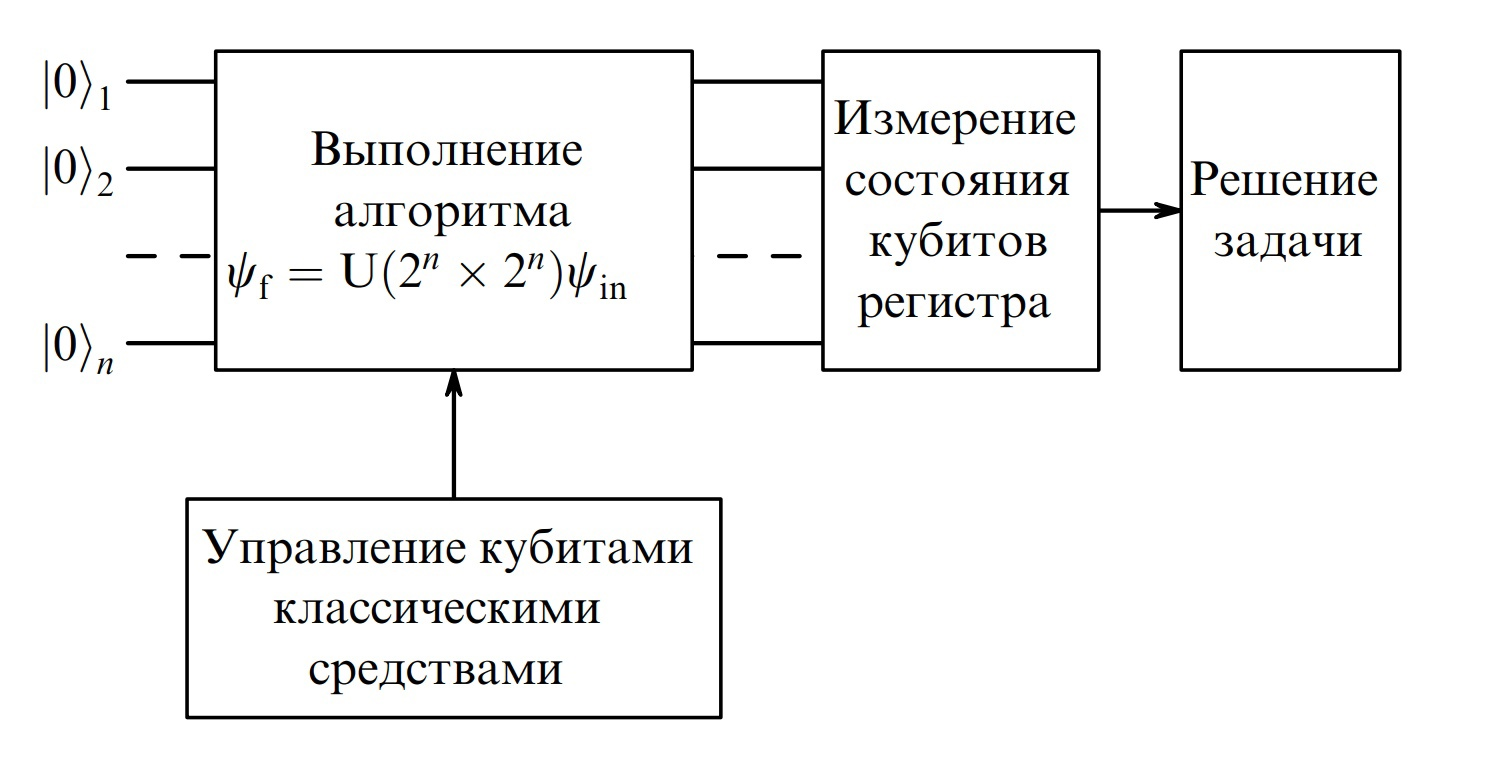
\includegraphics[scale=0.165]{3figure.jpg}}
        \end{minipage}\\
        \vspace{0.3cm}
        \footnotesize{\textbf{Рисунок 13.} Схема квантового компьютера.}
    \end{flushleft}
    \normalsize{
    Назовем \emph{идеальным} квантовый компьютер, состояния которого всегда когерентны. Это означает, во-первых, отсутствие взаимодействия компьютера
    с окружением, создающим шумы и нарушающим когерентность вектора состояния компьютера (декогерентизация); во-вторых, в идеальном квантовом компьютере
    внешние сигналы осуществляют точное управление.

    Вектор состояния $\vert\psi\rangle$ квантового регистра из $n$ кубитов
    представляет собой \emph{разложение} по $2^n$ базисным состояниям регистра $\vert i_1 \ldots i_n \rangle, i_1, \ldots, i_n = \{0, 1\}:$
    \begin{equation}
        \vert\psi\rangle=\sum\limits_{i_1,\ldots,i_n}a_{i_1,\ldots,i_n}\vert i_1\ldots i_n\rangle.
    \end{equation}
    Здесь суперпозиция $\vert\psi\rangle$ является вектором в $2^n$-мерном векторном пространстве, \(\vert i_1\ldots i_n\rangle\)~--- $2^n$ базисных векторов (ортов) этого пространства, $a_{i_1,\ldots,i_n}$~--- проекции вектора $\vert\psi\rangle$ на направления ортов $\vert i_1 \ldots i_n \rangle$.
    Все, что можно сделать с системой,~--- это преобразовать ее начальный вектор состояния $\vert\psi_{in}\rangle$ в другой вектор: $\vert\psi_f\rangle$. Поэтому процесс вычислений на квантовом компьютере рассматривается как преобразование начального вектора состояния компьютера $\vert\psi_{in}\rangle$ в конечный вектор состояния $\vert\psi_f\rangle$ путем умножения вектора $\vert\psi_{in}\rangle$ на унитарную матрицу $U$ размерности $2^n \times 2^n$:
    \begin{equation}
        \vert\psi_f\rangle=U(2^n\times 2^n)\vert\psi_{in}\rangle.
    \end{equation}
    Удобно полагать, что в начальном состоянии компьютера все его кубиты находятся в состоянии $\vert0\rangle$:
    \begin{equation}
        \vert\psi_{in}\rangle=\vert0_1\ldots 0_n\rangle.
    \end{equation}
    Эту операцию называют инициализацией. Состояние $\vert0_1\ldots 0_n\rangle$ можно получить или с помощью глубокого охлаждения (до температур порядка миликельвина), или путем применения методов поляризации.
    
    Алгоритм решения задачи заключен в матрице преобразования $U(2^n\times 2^n).$ Классическая информация о решении задачи содержится в конечном векторе состояния $\vert\psi_f\rangle$; она должна быть получена измерением кубитов.

    Для решения задачи на квантовом компьютере необходимо изготовить необходимое количество кубитов, инициализировать их, управлять их квантовой эволюцией, выполнить преобразование $U\vert\psi_{in}\rangle$ и измерить состояния кубитов, описываемых вектором $\vert\psi_f\rangle=U\vert\psi_{in}\rangle.$
    }\\
    \section*{Взгляд в будущее}
    \normalsize{
        На сегодняшний день квантовые компьютеры производятся, например, в октябре корпорация \emph{Google} заявила, что добилась квантового превосходства~--- 54-кубитный квантовый процессор \emph{Sycamore} сумел превзойти один из мощнейших в мире суперкомпьютеров \emph{Summit} разработки \emph{IBM}
        в задаче генерации случайных числовых строк, выполнив ее за 200 секунд, тогда как у классического суперкомпьютера на это ушло бы $10~000$ лет.
        
        Кроме того, существует квантовый процессор \emph{D-Wawe Advantage} на 5760 кубитов, однако он может решать лишь ограниченный круг задач.

        Допустим, придет время, когда будет освоена квантовая динамика систем на атомном уровне и построена квантовая информационная техника. Что дальше? Какие новые ресурсы природы могут быть использованы
        для создания новых поколений информационной техники? Степени свободы систем в меньших, чем атом, объемах (атомные ядра, элементарные частицы) связаны с большими энергиями, что затрудняет их использование для кодирования информации.
        Означает ли это, что на атомном уровне будут исчерпаны информационные ресурсы природы?
    }\\
    \section*{Список литературы}
    \small{
    $\cdot$ Michael A. Nielsen, Isaac L. Chuang \href{http://mmrc.amss.cas.cn/tlb/201702/W020170224608149940643.pdf}{Quantum Computation and Quantum Information.} 10th Anniversary Edition. 2010.\\
    $\cdot$ Килин С. Я. \href{https://web.archive.org/web/20100929192824/http://ufn.ru/ru/articles/1999/5/b/}{Квантовая информация}, май 1999 г.~--- Т. 169. № 5~--- С. 507-527.\\
    $\cdot$ Валиев К. А. \href{https://ufn.ru/ru/articles/1999/6/i/}{Квантовые компьютеры: можно ли их сделать <<большими>>?}~--- 1999. Т. 169. № 6~--- С. 691-694.\\
    $\cdot$ Валиев К. А. \href{https://ufn.ru/ru/articles/2005/1/a/}{Квантовые компьютеры и квантовые вычисления.}~--- 2005.~--- Т. 175.~--- С. 3-39.\\
    $\cdot$ A. M. Steane, E. G. Rieffel. \href{https://web.archive.org/web/20061017015251/http://www.fxpal.com/?p=abstract&abstractID=50}{Beyond Dits: The Future of Quantum Information Processing.}~--- January 2000.~--- P. 38-45.\\
    $\cdot$ \href{http://psj.nsu.ru/lector/neizvestniy/}{Квантовый компьютер и его полупроводниковая база.} 08.04.2003.
    }
\end{multicols}